\documentclass[11pt,aspectratio=169]{beamer}

% ============================================================
%  Master's Seminar Slides
%  Predicting Catastrophic Overfitting in Fast Adversarial Training
%  Author: Farzan Rahmani
% ============================================================

\usetheme{Madrid}
\usecolortheme{whale}

\usepackage[utf8]{inputenc}
\usepackage[T1]{fontenc}
\usepackage{amsmath,amssymb}
\usepackage{graphicx}
\usepackage{booktabs}
\usepackage{hyperref}
\usepackage{caption}

\graphicspath{{./images/}}

% ---------- Colors (Sharif-style navy/blue) ----------
\definecolor{sharifblue}{RGB}{0,51,102}
\setbeamercolor{structure}{fg=sharifblue}
\setbeamercolor{title}{fg=white,bg=sharifblue}
\setbeamercolor{frametitle}{fg=white,bg=sharifblue}
\setbeamercolor{palette primary}{fg=white,bg=sharifblue}
\setbeamercolor{palette secondary}{fg=white,bg=sharifblue!80}
\setbeamercolor{palette tertiary}{fg=white,bg=sharifblue!60}

% ---------- Footline with page numbers ----------
\setbeamertemplate{footline}{%
  \leavevmode%
  \hbox{%
  \begin{beamercolorbox}[wd=.55\paperwidth,ht=2.5ex,dp=1.125ex,leftskip=.3cm]{author in head/foot}%
    \usebeamerfont{author in head/foot}\insertshortauthor
  \end{beamercolorbox}%
  \begin{beamercolorbox}[wd=.30\paperwidth,ht=2.5ex,dp=1.125ex,center]{title in head/foot}%
    \usebeamerfont{title in head/foot}\insertshorttitle
  \end{beamercolorbox}%
  \begin{beamercolorbox}[wd=.15\paperwidth,ht=2.5ex,dp=1.125ex,right,rightskip=.3cm]{date in head/foot}%
    \usebeamerfont{date in head/foot}\insertframenumber{} / \inserttotalframenumber
  \end{beamercolorbox}}%
}

% ---------- Logo on content slides (top-right corner) ----------
% Replace "logo" with the path/filename of your university logo image
\logo{
\includegraphics[height=0.8cm]{logo}}

\setbeamertemplate{navigation symbols}{}
\setbeamertemplate{caption}[numbered]

% ---------- Title / author metadata ----------
\title[Predicting Catastrophic Overfitting in FAT]{Predicting Catastrophic Overfitting \\ in Fast Adversarial Training}
\subtitle{Master's Seminar -- AI and Robotics Track}
\author[F. Rahmani]{Farzan Rahmani}
\institute[Sharif University of Technology]{
  Department of Computer Engineering \\
  Sharif University of Technology
}
\date{July 2026}

\begin{document}

% ============================================================
\begin{frame}[plain]
  \begin{center}
    
\includegraphics[height=2cm]{logo}\\[0.4cm]
    {\small Sharif University of Technology \\ Department of Computer Engineering}\\[0.15cm]
    {\small Master's Seminar -- AI and Robotics Track}\\[0.6cm]
    {\Large\bfseries Predicting Catastrophic Overfitting \\ in Fast Adversarial Training}\\[0.8cm]
    \begin{tabular}{ll}
      \textbf{Presented by:} & Farzan Rahmani (403210725) \\[0.15cm]
      \textbf{Email:} & \texttt{farzan.rahmani@ce.sharif.edu} \\[0.3cm]
      \textbf{Supervisor:} & Dr. Mohammad Hossein Rohban \\[0.15cm]
      \textbf{Internal Examiner:} & Dr. Shohreh Kasaei \\
    \end{tabular}
    \vfill
    {\small July 2026}
  \end{center}
\end{frame}

% ============================================================
\begin{frame}{Outline}
  \tableofcontents
\end{frame}

% ============================================================
\section{Introduction}

\begin{frame}{Adversarial Examples}
  \begin{columns}[T]
    \begin{column}{0.55\textwidth}
      \begin{itemize}
        \item Deep neural networks achieve remarkable performance across vision, NLP, and autonomous systems.
        \item However, they are highly vulnerable to \textbf{adversarial attacks}: small, often imperceptible perturbations that flip predictions with high confidence \cite{szegedy2014intriguing}.
        \item This vulnerability raises serious concerns for safety-critical applications.
      \end{itemize}
    \end{column}
    \begin{column}{0.45\textwidth}
      \centering
      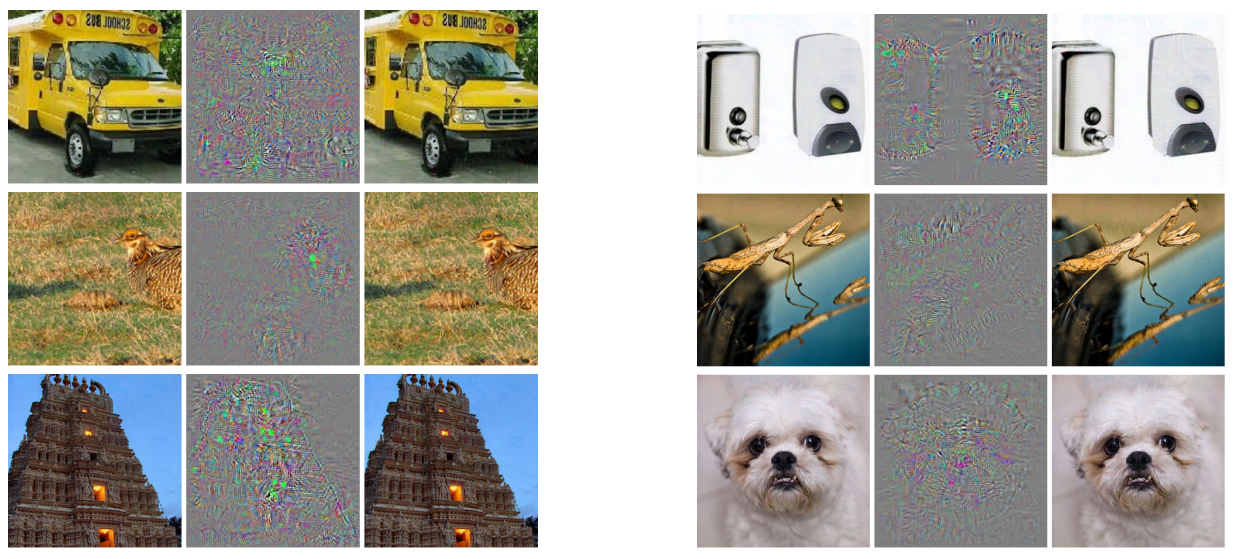
\includegraphics[width=\linewidth]{adversarial_examples.png}
      \captionof{figure}{Adversarial example for AlexNet \cite{krizhevsky2012imagenet,szegedy2014intriguing}}
    \end{column}
  \end{columns}
\end{frame}

\begin{frame}{Problem Definition}
  \begin{itemize}
    \item \textbf{Adversarial Training (AT)}: the leading defense; trains on adversarially perturbed samples instead of clean data \cite{madry2018towards}.
    \item Multi-step AT (e.g., PGD) is effective but \textbf{computationally expensive} -- limits scalability.
    \item \textbf{Fast Adversarial Training (FAT)} uses single-step attacks (e.g., FGSM) to reduce cost \cite{wong2020fast}.
    \item FAT suffers from \textbf{Catastrophic Overfitting (CO)}: robust accuracy against multi-step attacks suddenly collapses to near zero after a few epochs, while single-step accuracy keeps rising.
  \end{itemize}
\end{frame}

\begin{frame}{Why Does This Matter?}
  \begin{itemize}
    \item Robustness is critical in security-sensitive applications: autonomous driving, medical diagnosis, finance.
    \item Multi-step AT is reliable but too costly for large-scale models/datasets.
    \item FAT is efficient, but \textbf{unreliable} until CO is solved.
    \item Most existing CO-prevention methods add expensive hyperparameter tuning or extra computation -- undermining FAT's original goal of cheap robustness.
  \end{itemize}
  \vskip 0.3cm
  \begin{block}{Goal of this seminar}
    Review key concepts and prior work on catastrophic overfitting, and introduce an early idea for \textbf{low-cost prediction} of CO and \textbf{dynamic step-size} adjustment.
  \end{block}
\end{frame}

% ============================================================
\section{Background}

\begin{frame}{Adversarial Attacks}
  \textbf{Fast Gradient Sign Method (FGSM)} \cite{goodfellow2015explaining}:
  \[
  \delta = \epsilon \cdot \mathrm{sign}\big( \nabla_{x} \mathcal{L}(f_{\theta}(x), y) \big)
  \]
  \vskip 0.2cm
  \textbf{Projected Gradient Descent (PGD)} \cite{madry2018towards}:
  \[
  x^{t+1} = \Pi_{\|x'-x\|_{\infty}\le\epsilon}\Big( x^{t} + \alpha \cdot \mathrm{sign}\big( \nabla_{x} \mathcal{L}(f_{\theta}(x^{t}), y) \big) \Big)
  \]
  \begin{itemize}
    \item $\epsilon$: perturbation radius (e.g., $8/255$) \quad $\alpha$: step size (e.g., $2/255$)
    \item PGD-10 / PGD-20: iterated for 10 / 20 steps $\rightarrow$ \textbf{robust accuracy}
  \end{itemize}
\end{frame}

\begin{frame}{Adversarial Training \& Fast AT}
  \textbf{Min-max formulation} \cite{madry2018towards}:
  \[
  \min_{\theta} \; \mathbb{E}_{(x,y)\sim\mathcal{D}} \left[ \max_{\|\delta\|_{\infty}\le\epsilon} \mathcal{L}(f_{\theta}(x+\delta), y) \right]
  \]
  \begin{itemize}
    \item Inner max: find worst-case perturbation. Outer min: update model to resist it.
    \item Standard AT solves the inner problem with multi-step PGD $\rightarrow$ up to $10\times$ training cost.
    \item \textbf{Fast AT} approximates the inner max with a \emph{single} FGSM step \cite{wong2020fast}.
    \item Adding a \textbf{random start} to the perturbation was found to improve stability.
  \end{itemize}
\end{frame}

\begin{frame}{Catastrophic Overfitting (CO)}
  \begin{columns}[T]
    \begin{column}{0.5\textwidth}
      \begin{itemize}
        \item After a few epochs of single-step FAT, \textbf{PGD robust accuracy collapses} to near zero.
        \item \textbf{FGSM accuracy} keeps increasing -- sometimes even above clean accuracy.
        \item The model overfits to the specific attack used in training rather than gaining true robustness.
      \end{itemize}
    \end{column}
    \begin{column}{0.5\textwidth}
      \centering
      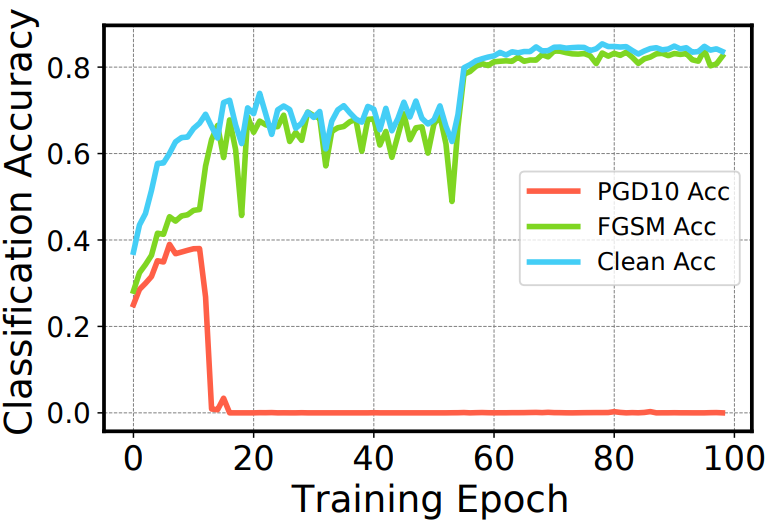
\includegraphics[width=\linewidth]{catastrophic_overfitting.png}
      \captionof{figure}{\tiny CO in FAT: clean / FGSM / PGD-10 accuracy over training \cite{wang2024preventing}}
    \end{column}
  \end{columns}
\end{frame}

\begin{frame}{Loss Landscape Distortion}
  \centering
  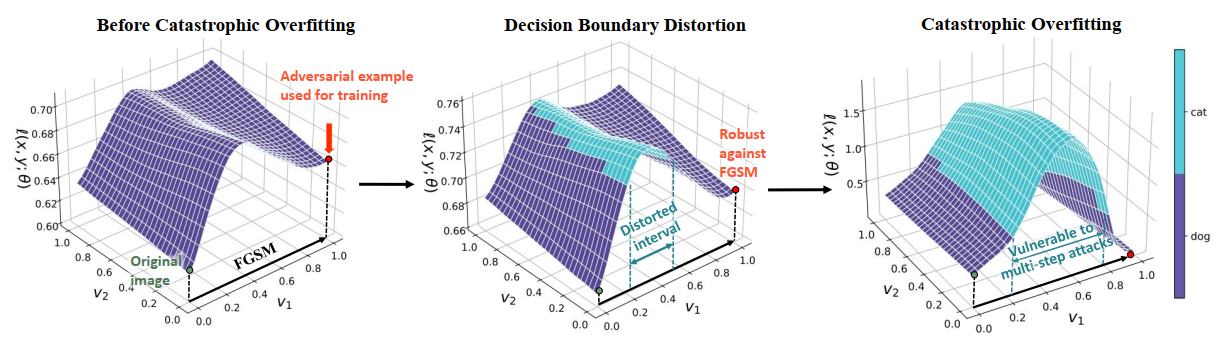
\includegraphics[width=0.85\linewidth]{loss_landscape_distortion.png}
  \captionof{figure}{\tiny Decision boundary distortion driving catastrophic overfitting \cite{kim2021understanding}}
  \begin{itemize}
    \item Before CO: loss surface is smooth; FGSM direction correctly points to high loss.
    \item As training proceeds, the loss surface becomes sharply \textbf{non-linear} near adversarial examples \cite{kim2021understanding,kang2021understanding}.
    \item FGSM can no longer approximate the true worst-case direction $\rightarrow$ robustness collapses.
  \end{itemize}
\end{frame}

\begin{frame}{Curvature, Second-Order View \& Evaluation}
  \begin{itemize}
    \item Smoother (lower-curvature) loss $\Rightarrow$ single-step attacks approximate the true maximum better.
    \item Second-order information (e.g., Hessian) is informative for CO but expensive to compute directly.
    \item \textbf{Evaluation}: FGSM accuracy alone is misleading; reliable evaluation uses strong multi-step attacks such as \textbf{AutoAttack} \cite{croce2020reliable}.
    \item Key trade-off: \textbf{robustness vs. clean accuracy} \cite{tsipras2019robustness}.
  \end{itemize}
\end{frame}

% ============================================================
\section{Prior Work}

\begin{frame}{Randomization-Based Methods}
  \begin{itemize}
    \item \textbf{FGSM-RS} \cite{wong2020fast}: random start before FGSM perturbation -- largely prevents CO but not always at larger $\epsilon$.
    \item \textbf{N-FGSM} \cite{dejorge2022make}: larger-magnitude random noise (radius $k > \epsilon$) with \emph{no clipping} $\rightarrow$ more diverse perturbations, better robustness.
  \end{itemize}
  \centering
  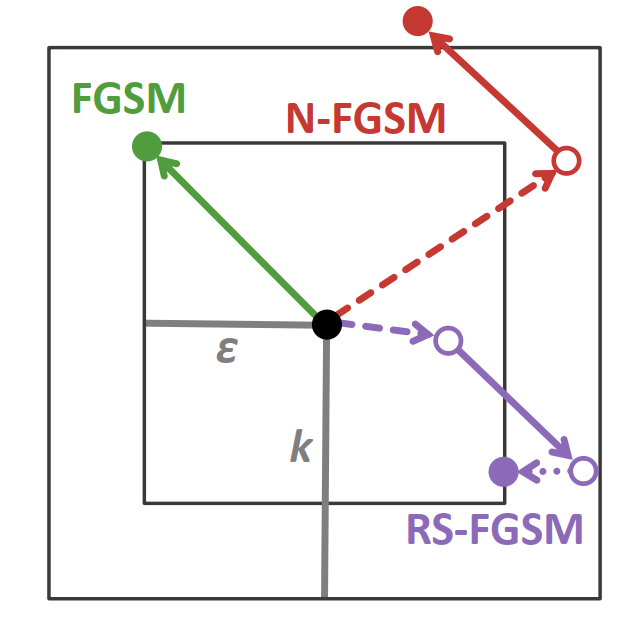
\includegraphics[width=0.25\linewidth]{nfgsm_comparison.png}
  \captionof{figure}{\tiny FGSM vs. RS-FGSM vs. N-FGSM \cite{goodfellow2015explaining,wong2020fast,dejorge2022make}}
\end{frame}

\begin{frame}{Regularization-Based Methods}
  \begin{itemize}
    \item \textbf{GradAlign} \cite{andriushchenko2020understanding}: maximizes gradient alignment between clean and perturbed samples.
    \item \textbf{NuAT} \cite{sriramanan2021towards}: nuclear-norm regularization to smooth the loss.
    \item \textbf{AAER} \cite{lin2023eliminating}: detects and regularizes \emph{abnormal adversarial examples}.
    \item \textbf{ELLE} \cite{rocamora2024efficient}: encourages local linearity of the loss surface efficiently.
  \end{itemize}
\end{frame}

\begin{frame}{Adaptive Step-Size \& Other Approaches}
  \textbf{Adaptive step size:}
  \begin{itemize}
    \item Reinforcement-learning-based step size \cite{nie2021adaptive}
    \item \textbf{ATAS} -- step size adapted via gradient norm \cite{huang2023fast}
    \item Per-sample step size from noise/gradient similarity \cite{zhao2025avoiding}
  \end{itemize}
  \textbf{Other approaches:}
  \begin{itemize}
    \item \textbf{ZeroGrad} \cite{golgooni2023zerograd}: drops updates with negligible gradient magnitude.
    \item \textbf{Free AT} \cite{shafahi2019adversarial}: reuses attack gradients for weight updates.
    \item \textbf{Curvature regularization} \cite{moosavi2019robustness}: directly controls loss curvature.
  \end{itemize}
\end{frame}

\begin{frame}{Prediction Metrics for CO}
  No metric has been designed \emph{purely} for low-cost CO prediction, but a few serve as indirect early signals:
  \vskip 0.15cm
  \textbf{Gradient Alignment} \cite{andriushchenko2020understanding}:
  \[
  \mathbb{E}\left[ \cos\big( \nabla_x \mathcal{L}(x,y;\theta),\, \nabla_x \mathcal{L}(x+\eta,y;\theta) \big) \right]
  \]
  \begin{itemize}
    \item Near 1 $\Rightarrow$ locally linear loss; sharp drop $\Rightarrow$ CO warning. \textbf{Costs an extra backward pass.}
  \end{itemize}
  \textbf{Abnormal Adversarial Examples (AAE)} \cite{lin2023eliminating}: samples where adding the FGSM perturbation \emph{decreases} the loss -- also costly to track (loss at two points).
\end{frame}

\begin{frame}{Limitations of Prior Work}
  \begin{enumerate}
    \item \textbf{Dataset/architecture dependence} -- tuned mainly for CIFAR-10-scale settings.
    \item \textbf{Hyperparameter tuning} required per dataset/architecture.
    \item \textbf{Extra computational cost} (e.g., GradAlign, ELLE).
    \item \textbf{No efficient prediction metric} exists that anticipates CO \emph{before} it happens at negligible cost.
  \end{enumerate}
  \vskip 0.2cm
  \begin{block}{Gap}
    No prior method simultaneously solves all four issues -- this motivates the approach explored next.
  \end{block}
\end{frame}

% ============================================================
\section{Proposed Direction}

\begin{frame}{Observation: Epsilon Overfitting}
  \begin{columns}[T]
    \begin{column}{0.5\textwidth}
      \begin{itemize}
        \item Trained PreActResNet18 on CIFAR-10 with fixed $\epsilon=8/255$ until CO occurred.
        \item Measured accuracy vs. attack strength ($-16/255$ to $+16/255$) for FGSM and PGD-10.
        \item FGSM accuracy is highly \textbf{erratic} across $\epsilon$ values; PGD-10 stays near zero throughout.
      \end{itemize}
    \end{column}
    \begin{column}{0.5\textwidth}
      \centering
      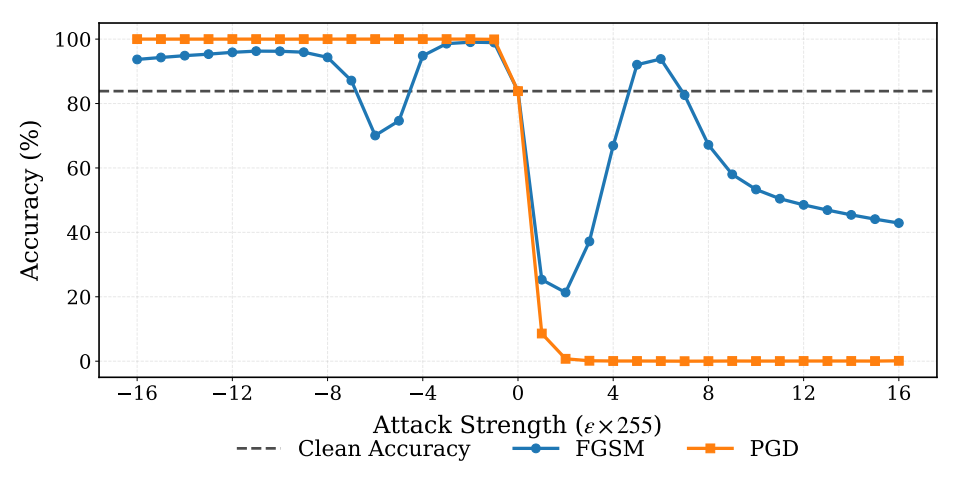
\includegraphics[width=\linewidth]{epsilon_overfitting_fgsm.png}
      \captionof{figure}{\tiny Accuracy vs. attack strength for a CO model}
    \end{column}
  \end{columns}
  \vskip 0.1cm
  \small $\rightarrow$ The model overfits to specific perturbation magnitudes (\textbf{``epsilon overfitting''}) rather than gaining true robustness -- motivating diversity in perturbation size/direction.
\end{frame}

\begin{frame}{Prediction Metric: Perturbation Alignment}
  \[
  \text{PertAlign} = \cos\!\Big( \nabla_{x} \mathcal{L}(f_{\theta}(x'), y),\; \nabla_{x} \mathcal{L}(f_{\theta}(x'+\delta), y) \Big)
  \]
  where $x' = x+\eta$, $\eta \sim \mathcal{U}([-\epsilon,\epsilon]^d)$, and $\delta$ is a small step in the attack direction.
  \begin{itemize}
    \item Near 1 $\Rightarrow$ locally linear loss; drops toward 0 near CO onset.
    \item \textbf{Key advantage}: both gradients are already computed during standard single-step AT $\Rightarrow$ \textbf{virtually no extra cost}.
  \end{itemize}
  \centering
  \includegraphics[width=0.55\linewidth]{perturbation_alignment_senet18_cifar10.png}
  \captionof{figure}{\tiny PertAlign drop precedes FGSM/PGD-10 divergence}
\end{frame}

\begin{frame}{Toward Dynamic Step-Size Adjustment}
  \begin{itemize}
    \item View the inner maximization through a \textbf{second-order (quadratic) local approximation} of the loss.
    \item Use the same gradients already computed for PertAlign to estimate a locally optimal step size -- \textbf{nearly free}.
    \item Combining: (1) diversified perturbation distribution, (2) low-cost CO prediction via PertAlign, and (3) dynamic step size $\rightarrow$ a method robust across datasets/architectures with a \textbf{fixed} hyperparameter set.
    \item Full method design and large-scale evaluation: \textbf{future thesis work}.
  \end{itemize}
\end{frame}

% ============================================================
\section{Conclusion}

\begin{frame}{Conclusion}
  \begin{itemize}
    \item Catastrophic overfitting is the main obstacle to efficient, reliable Fast Adversarial Training.
    \item Reviewed core concepts (attacks, AT, FAT, CO) and their link to loss-landscape curvature.
    \item Surveyed prior work: randomization, regularization, adaptive step size, and other strategies -- each partially effective, none solving all four key limitations.
    \item Preliminary evidence presented:
    \begin{itemize}
      \item \textbf{Epsilon overfitting} phenomenon in FGSM accuracy.
      \item \textbf{PertAlign} metric providing an early, near-free warning signal for CO.
    \end{itemize}
    \item Next step: full design and evaluation of a low-cost, dynamic-step-size FAT method.
  \end{itemize}
\end{frame}

% ============================================================
\section{References}

\begin{frame}[allowframebreaks]{References}
  \footnotesize
  \begin{thebibliography}{99}
    \bibitem{szegedy2014intriguing} Szegedy et al., ``Intriguing Properties of Neural Networks,'' ICLR, 2014.
    \bibitem{krizhevsky2012imagenet} Krizhevsky et al., ``ImageNet Classification with Deep CNNs,'' NeurIPS, 2012.
    \bibitem{goodfellow2015explaining} Goodfellow et al., ``Explaining and Harnessing Adversarial Examples,'' ICLR, 2015.
    \bibitem{madry2018towards} Madry et al., ``Towards Deep Learning Models Resistant to Adversarial Attacks,'' ICLR, 2018.
    \bibitem{wong2020fast} Wong et al., ``Fast is Better than Free: Revisiting Adversarial Training,'' ICLR, 2020.
    \bibitem{wang2024preventing} Wang et al., ``Preventing Catastrophic Overfitting in Fast AT,'' ECCV, 2024.
    \bibitem{andriushchenko2020understanding} Andriushchenko \& Flammarion, ``Understanding and Improving Fast Adversarial Training,'' NeurIPS, 2020.
    \bibitem{dejorge2022make} de Jorge et al., ``Make Some Noise: Reliable and Efficient Single-Step AT,'' NeurIPS, 2022.
    \bibitem{lin2023eliminating} Lin et al., ``Eliminating Catastrophic Overfitting via Abnormal Adversarial Examples Regularization,'' NeurIPS, 2023.
    \bibitem{rocamora2024efficient} Rocamora et al., ``Efficient Local Linearity Regularization to Overcome CO,'' ICLR, 2024.
    \bibitem{shafahi2019adversarial} Shafahi et al., ``Adversarial Training for Free!,'' NeurIPS, 2019.
    \bibitem{golgooni2023zerograd} Golgooni et al., ``ZeroGrad: Costless Conscious Remedies for CO,'' Intelligent Systems with Applications, 2023.
    \bibitem{huang2023fast} Huang et al., ``Fast Adversarial Training with Adaptive Step Size,'' IEEE TIP, 2023.
    \bibitem{sriramanan2021towards} Sriramanan et al., ``Towards Efficient and Effective Adversarial Training,'' NeurIPS, 2021.
    \bibitem{moosavi2019robustness} Moosavi-Dezfooli et al., ``Robustness via Curvature Regularization, and Vice Versa,'' CVPR, 2019.
    \bibitem{tsipras2019robustness} Tsipras et al., ``Robustness May Be at Odds with Accuracy,'' ICLR, 2019.
    \bibitem{croce2020reliable} Croce \& Hein, ``Reliable Evaluation of Adversarial Robustness with AutoAttack,'' ICML, 2020.
    \bibitem{kim2021understanding} Kim et al., ``Understanding Catastrophic Overfitting in Single-Step AT,'' AAAI, 2021.
    \bibitem{kang2021understanding} Kang \& Moosavi-Dezfooli, ``Understanding Catastrophic Overfitting in Adversarial Training,'' arXiv:2105.02942, 2021.
    \bibitem{zhao2025avoiding} Zhao et al., ``Avoiding CO in Fast AT with Adaptive Similarity Step Size,'' PLOS ONE, 2025.
    \bibitem{nie2021adaptive} Nie et al., ``Adaptive Perturbation Adversarial Training: Based on RL,'' arXiv:2108.13239, 2021.
  \end{thebibliography}
\end{frame}

% ============================================================
\begin{frame}[plain]
  \begin{center}
    \Huge\bfseries Thank You!
    \vskip 1cm
    \Large Questions \& Discussion
    \vskip 1.5cm
    \normalsize
    Farzan Rahmani \\
    \texttt{farzan.rahmani@ce.sharif.edu}
  \end{center}
\end{frame}

\end{document}
